\chapter{TYTUŁ ROZDZIAŁU PIERWSZEGO}

{%\markboth{}{}
%\setlength{\parskip}{1.2ex plus 0.5ex minus 0.2ex}
%\baselineskip 0.6cm

%\lipsum % usunąć linię
\section{Numerowanie}
\textit{To czcionka       pochylona}. \\
Tekst piszemy standardowo nie przejmując się ilością spacji Tekst pierwszego rozdziału  aa
ma spełniać dwa warunki:
\begin{itemize}
    \item warunek 1 hgi;ghasioga kjabsgkjasb sakgjbas;kjbas askgbasd;kgasbgb;a sdvafd afd ad fb afdb daf b adfb afd bad fb adf
    \item war2
\end{itemize}
\subsection{nowe}
\begin{itemize}
	\item[$\star$] tuygfasgl
	\item[$\star$] ksdbvalskval
\end{itemize}
\begin{enumerate}
	\item warunek 2
	\item warynenckjd
\end{enumerate}

\section[skrót]{Wzory matematyczne}
W tekście wzory piszemy następująco $wzor$ i już. $y=x_{11}^2$ $x_{132425}^{ads}$

Wzór wyeksponowany

nienumerowany
$$
F(x)=\sqrt{x_1^3}
$$

numerowany
\begin{equation}
	\label{eq: wczesniej}
	x^2
\end{equation}

\begin{equation}
	\label{eq:cos} %etykieta wzoru
	F(x)=\frac{x_1^2}{\sqrt{2x-4}}
\end{equation}
We wzorze \eqref{eq:cos} należy coś zrobić

Granice wyrażeń
$$
\lim\limits_{x\rightarrow \infty} \frac{x-3}{x^2+5}
$$

$f'(x), f''(x), f'''(x),\ \ \  f^{(iv)}(x)$

$$
\sum_{i=1}^{\infty} \frac{i}{i+1}
$$

$$
\int f(x) dx ,\ \ \int_{1}^{3} f(x) dx \ \ \ \int\limits_5^6 f(x) dx \ \ 
\iint f(x) \iiint\limits_{1}^3
$$

$x\in \mathbb{R, N, Z, C}$ 

$x\notin R$

Kroje pisma standardowy, \textit{kursywa}, \textbf{wytłuszczenie}, \underline{podkreślenie} \textcolor{green}{tekst kolorowy}

Kroje pisma matematycznego $standard\ to\ kursywa $, $\mathrm{tekst}$, $\mathbf{pogrubiony}$  $\mathcal{kaligrafia}$

$$
x>0, x<0, x\geq 0, x\le 0, x\leqq 7
$$

Równania wielowierszowe
\begin{equation*}
	f(x)=\left(\frac{\frac{1}{x+3}}{x-4}\right)
\end{equation*}
%http://www.latex-kurs.x25.pl/paper/wyrazenia_matematyczne
$$
\left[
\begin{array}{cccc}
	a_{11} & a_{22} & \cdots & a_{33} \\
	a_{21} & a_{22} & \ddots & a_{23} \\
	a_{31} & a_{32} & \ldots & \vdots
\end{array}
\right]_{n\times n}
$$

\begin{equation*}
	f(x)=\left\{ \begin{array}{cl}
		x, & \text{gdy } x\geq 0,\\
		-x, & x<0.			
	\end{array}
	\right.
\end{equation*}

\begin{eqnarray}
	f(x) & = & \cos x \\
	f'(x) & = & -\sin x \\
	\int_{0}^{x} f(y)dy &
	= & \sin x
\end{eqnarray}


\begin{eqnarray}
	f(x) & = & \cos x  sdxse ef e f ef e fe f e fe f+ fw- fe + \nonumber\\
	 &  & -\sin x 
\end{eqnarray}

\begin{multline}
	a+b+c+d+e+f+g+h+i+j+k+\\
	l+m+n+o+p+q+r+s+t+w+x+y+z\\
	l+m+n+o+p+q+r+s+t+w+x+y+z
\end{multline}



Przykład tabeli
\begin{table}
\label{tab:numer}
\begin{center}
\begin{tabular}{ |c |c| l| }
\hline
 cell1 & cell2 & cell3 \\ 
 \hline\hline
 cell4 & c5 & ce \\ 
 \hline
 cell7 & cell8 & cell9  \\ 
 \hline
\end{tabular}
\end{center}
\caption{Podpis tabeli}
\end{table}

Przykład rysunku
\begin{figure}%[!b]
	\centering \includegraphics[width=0.9\textwidth]{img/Ti-xy3-3x2_kopia.jpg}
	\caption{Logo UR.}
\label{figure_1a}
\end{figure}

\begin{figure}%[!h]
	\centering 
	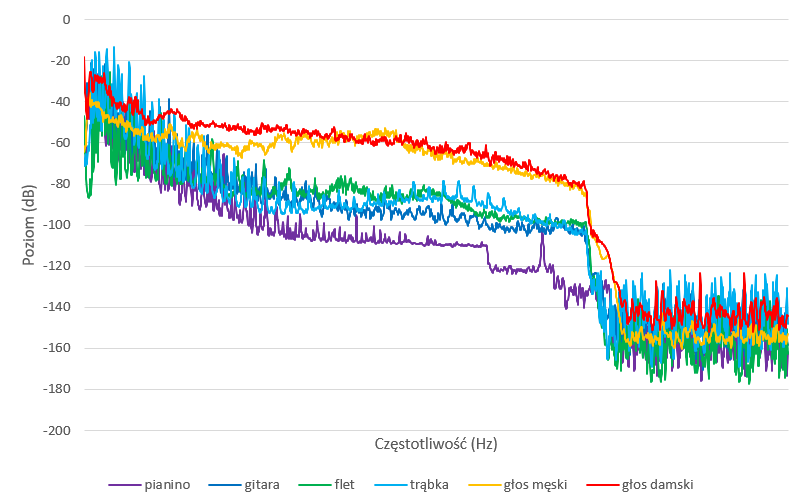
\includegraphics[trim= 0 0 150 150, clip, angle=45, width=0.9\textwidth]{wykres.png}
	\caption{Dziwny wykres}
\label{figure_1b}
\end{figure}

To jest {\textbf{grube}} a to jest \textit{pochyłe}


}